\documentclass{article}

\usepackage{fullpage}  % Makes the text margins smaller
\usepackage{graphicx} % To include figures
\usepackage{fancyvrb} % Includes the \VerbatimInput command to read in code files
\usepackage{amsmath}
\DeclareGraphicsExtensions{.png}
\renewcommand*{\arraystretch}{2}

\author{Cody Lieu, Yixin Lin}
\title{COMPSCI 527 Homework 6}

\begin{document}
\maketitle

% How to include pictures with captions
% 
% \begin{figure}[h!]
%   \caption{caption}
%   \centering
% 	\includegraphics{filename}
% \end{figure}


\section{Introduction}

3D object reconstruction from a set of 2D images is fundamentally an ill-conditioned problem, due to its inverse nature. We investigate the effects of noise and other parameters on the success of reconstructing the original 3D object from stereo images. We quantify the correctness of the reconstructed 3D object by measuring three types of errors: motion, structure, and reprojection error.

Our goal in this paper is to investigate the following questions:
\begin{itemize}
\item Which types of error fail first when enough noise is added for the shape to be unrecognizable? More generally, how does varying the image noise affect the different types of errors?

\item What happens when we change the image resolution but keep \texttt{sigma} fixed?
\end{itemize}

\newpage
\section{Progression of failure with increasing levels of noise}

% Explanation of problem
\subsection{Introduction}

The software provided creates a simulated world with a square object (with multiple colored squares on each side) and two cameras, adds Gaussian noise to the image coordinates, and runs the eight-point algorithm for 3-d reconstruction. Because reconstruction is a ill-conditioned/ill-posed problem (due to its inverse nature), small errors in the data will often result in large errors in the 3D reconstruction. 

We investigate the effect of pseudo-random Gaussian noise on different types of errors, especially as the image become so distorted that the reconstructed shape becomes unrecognizable.

We have three broad categories of errors:

\begin{enumerate}
  \item Motion error: the difference between true and computed motion, for both translation and rotation, measured in degrees
  \item Structure error: the difference between true and computed structure, measured in RMS average percentage error of the overall size of the object
  \item Reprojection error: the difference between the image of the original object and reprojected image of the reconstructed object, measured in RMS pixels per point
\end{enumerate} 

We pose the question: at the point where enough noise has been added so that the reconstructed object is unrecognizable, what types of errors fail first?

% Hypothesis

% \subsection{Hypothesis}

% Experiment ran

\subsection{Methods}

The experiment we ran was to run the following procedure, in which a subroutine was applied on a range of \texttt{sigma}s from \texttt{0:.25:5}, with n = 150 for each \texttt{sigma}; we recorded the average errors for each, as shown in Figures 1-3.

\subsection*{Procedure}

\begin{enumerate}
  \item Create a 3D world, with object (Gaussian noise \texttt{sigma} = 0), two cameras, and the resulting images
  \item Compute the true transformation between the camera reference frames
  \item Compute the true structure
  \item Subroutine for each \texttt{sigma} in range \texttt{0:.25:4}
  \begin{itemize}
  	\item Add noise to the original image with \texttt{sigma}
  	\item Compute the resulting transformation figure
  	\item Measure and record motion, structure, and reprojection errors
  \end{itemize}
\end{enumerate} 

After this, we also drew the reconstructed figures for choice \texttt{sigma} (Figures 4-9), to demonstrate the effects of noise on the resulting reconstruction and to find out when the reconstructed object became unrecognizable.

% Error plots (results)
% INCLUDE UNITS

\newpage
\subsection{Data}
\begin{center}
	\begin{center}Figure 1. Motion error\end{center}
	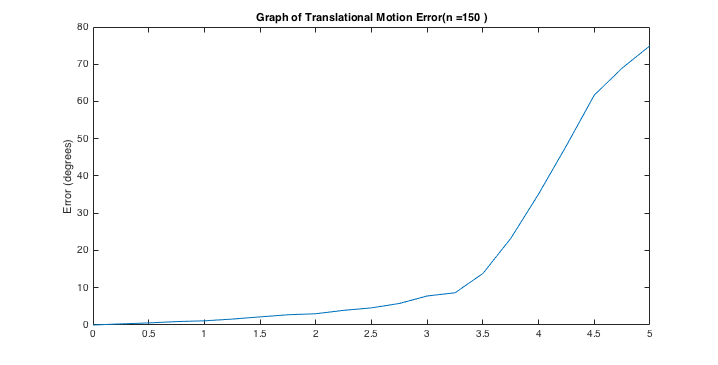
\includegraphics[width=.7\textwidth,keepaspectratio]{translation_motion_error.png}
	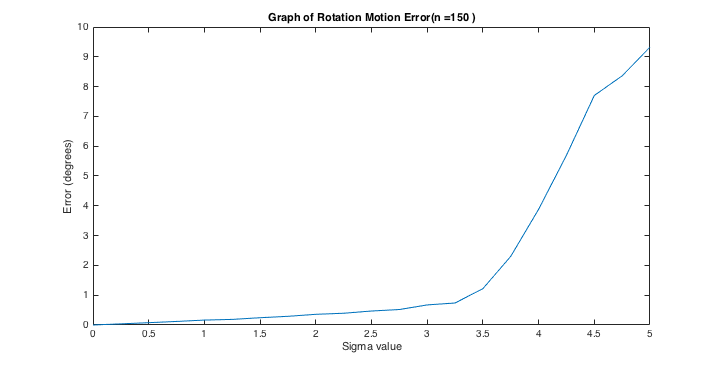
\includegraphics[width=.7\textwidth,keepaspectratio]{rotation_motion_error.png}
	\begin{center}Figure 2. Structure error\end{center}
	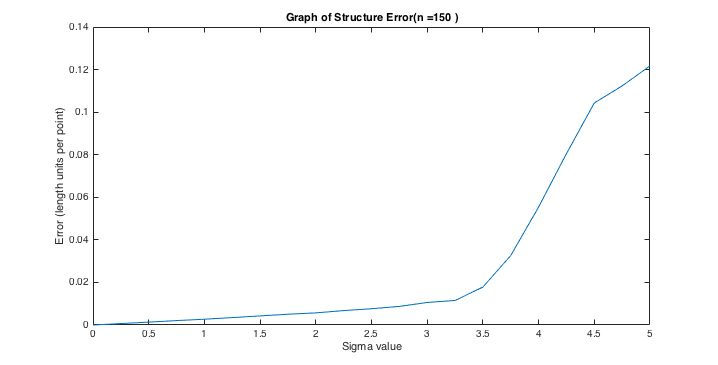
\includegraphics[width=.7\textwidth,keepaspectratio]{structure_error.png}
	\newpage

	\begin{center}Figure 3. Reprojection error\end{center}
	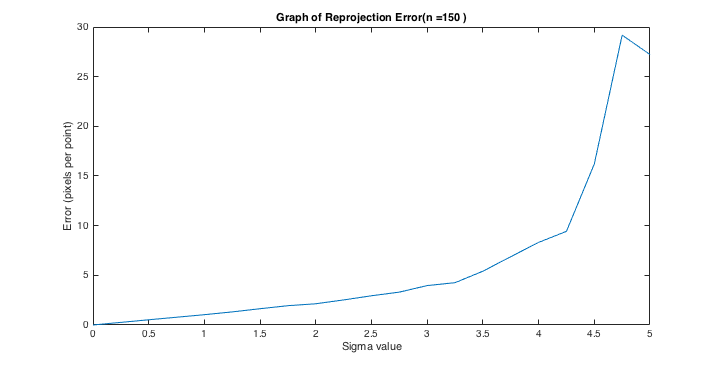
\includegraphics[width=.7\textwidth,keepaspectratio]{reprojection_error.png}

	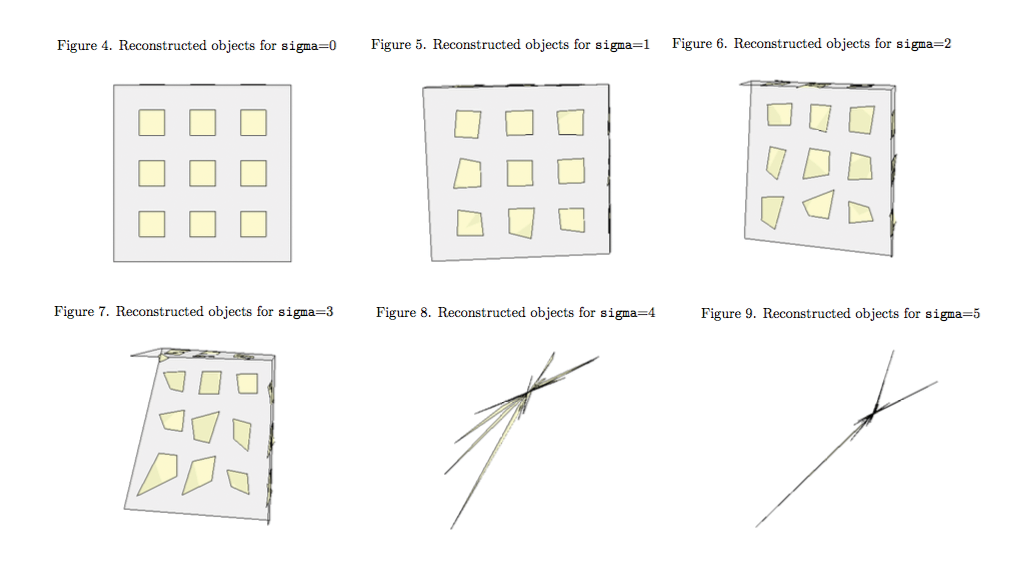
\includegraphics[width=\textwidth,keepaspectratio]{reconstructed_objects.png}
\end{center}

% Conclusions

\subsection{Conclusions}

Clearly, there is a severe drop in quality of the reconstructed object after \texttt{sigma} reaches around 3.25, and the reconstructed object for \texttt{sigma}=4 (Figure 8) is completely unrecognizable.

As we can see from the error plots, there is an inflection point around 3.25 where motion error (especially translation error) begins to climb drastically. This is followed immediately by structure error, which also has a similar inflection point. Finally, there is a slight inflection point in reprojection error, which is relatively delayed compared to the other errors (around \texttt{sigma}=4.25).

Interestingly, all of the error rates drop at around \texttt{sigma}=2.7, which is especially pronounced in translation motion and reprojection errors.

% Things learned

% Problems/ things to learn





\newpage
\section{Effects of modifying image resolution}

\newpage
\section{Conclusion}

\newpage


\newpage
\begin{thebibliography}{99}
\bibitem{hartley}
	Hartley, Richard. ``In defense of the eight-point algorithm.'' Pattern Analysis and Machine Intelligence, IEEE Transactions on 19, no. 6 (1997): 580-593.

\bibitem{chojnacki}
	Chojnacki, Wojciech, and Michael J. Brooks. ``On the consistency of the normalized eight-point algorithm.'' Journal of Mathematical Imaging and Vision 28, no. 1 (2007): 19-27.
\end{thebibliography}


\end{document}